\chapter{Composition}

\section{Linked Lists}
\begin{itemize}
    \item Linked list structure: a linked list is either empty or a first value and the rest of the linked list
    \item Linked lists are mutable
    \medskip
	\begin{figure}[H]
	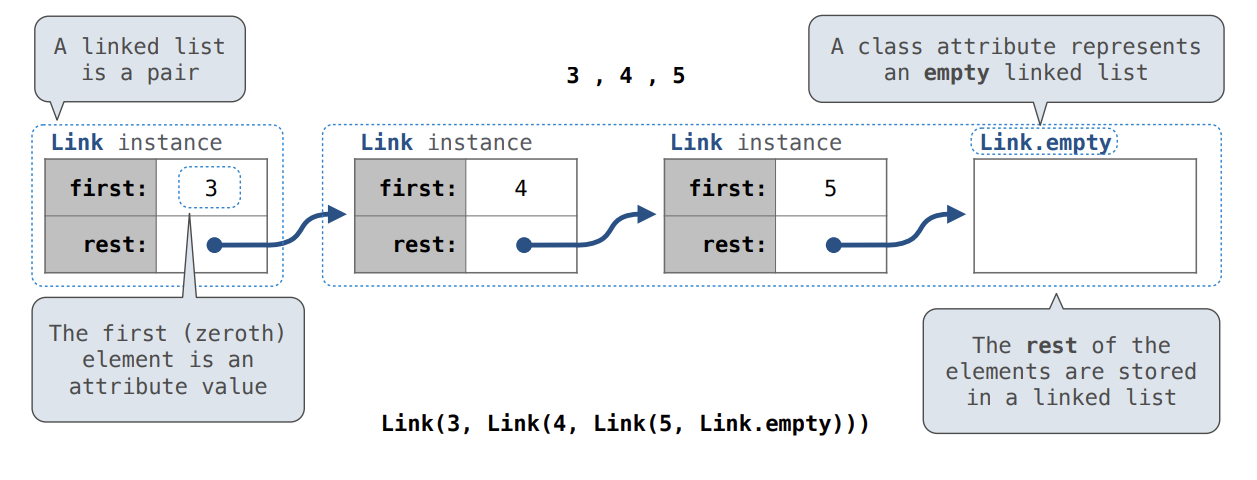
\includegraphics[width=1\linewidth]{figures/linked_list_example.png}
	\caption{Linked List Example}
	\end{figure}
\end{itemize}
\begin{minted}[tabsize=4]{Python}
    class Link:
        empty = () # some zero-length sequence
        def __init__(self, first, rest=empty):
            assert rest is Link.empty or isinstance(rest, Link) # verify rest is a linked list
            self.first = first
            self.rest = rest
\end{minted}

\section{Trees}
\begin{itemize}
    \item Recursive description of trees
    \begin{itemize}
        \item A tree has a root label and a list of branches
        \item Each branch is a tree
        \item A tree with zero branches is called a leaf
        \item A tree starts at the root
    \end{itemize}
    \item Relative description of trees
    \begin{itemize}
        \item Each location in a tree is called a node
        \item Each node has a label that can be any value
        \item One node can be the parent/child of another
        \item The top node is the root node
    \end{itemize}
    \item Tree processing often uses recursion, with the leaf as a base case
    \item Example tree implementation:
\end{itemize}
\begin{minted}[tabsize=4]{Python}
    class Tree:
        def __init__(self, label, branches=[]):
            self.label = label
            for branch in branches:
                assert isinstance(branch, Tree)
            self.branches = list(branches)
            for branch in branches:
        def tree(label, branches=[]):
            for branch in branches:
                assert is_tree(branch)
            return [label] + list(branches)
        def label(tree):
            return tree[0]
        def branches(tree):
            return tree[1:]
\end{minted}
\begin{itemize}
    \item Pruning: removing subtrees from a tree
    \item Pruning can be used before recursive processing to speed up computation
\end{itemize}

\section{Modular Design}
\begin{itemize}
    \item A design principle: isolate different parts of a program that address different concerns
    \item Each modular component can be developed and tested independently
    \item Example:
    \medskip
	\begin{figure}[H]
	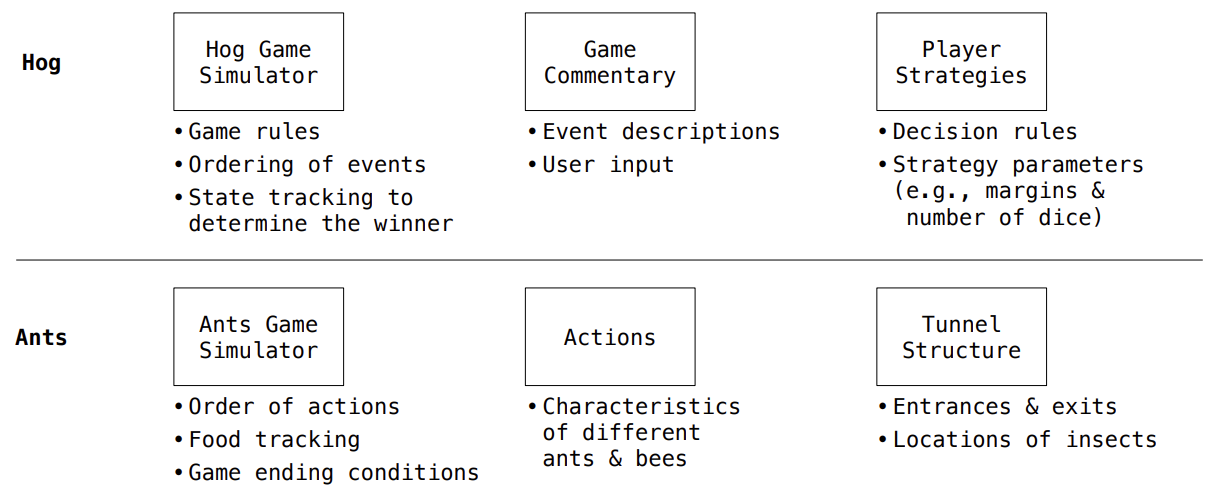
\includegraphics[width=1\linewidth]{figures/modular_design_example.png}
	\caption{Modular Design Example}
	\end{figure}
\end{itemize}